\documentclass{article}
\usepackage{amsmath}
\usepackage[margin=0.75in]{geometry}

\title{Detailed Explanations of Monetary Policy Concepts \\ \large Video Assignment Two}
\author{Charles Ancel}
\date{\today}

\begin{document}

\maketitle

\section{Federal Reserve's Process for Implementing Monetary Policy}
\textbf{Question: Explain the actual process the Federal Reserve takes to implement monetary policy.}

\subsection{Main Instrument of the Fed's Monetary Policy}
The main instrument of the Fed's monetary policy is the federal funds rate, which is the interest rate at which banks lend reserves to each other overnight. This rate is influenced through open market operations but is not directly controlled by the Fed.

\subsection{Decision Process in FOMC Meetings}
Monetary policy is decided in the Federal Open Market Committee (FOMC) meetings, where members review economic data, consider forecasts, and discuss economic conditions before voting on the appropriate level for the federal funds rate.

\subsection{Public Announcement}
The monetary policy decision is announced to the public via press releases and statements from the Fed, providing transparency and managing market expectations.

\subsection{Implementation by the New York Fed’s Open Market Trading Desk}
The New York Fed's Open Market Trading Desk implements the FOMC's decision by conducting open market operations, buying or selling government securities to influence the supply of reserves in the banking system.

\section{Objectives of Monetary Policy}
\textbf{Question: What are the (main) objectives of monetary policy?}

\subsection{Price Stability}
One of the main objectives of monetary policy is to maintain price stability, which means keeping inflation low and stable.

\subsection{Full Employment}
Another objective is to achieve full employment, where all who are willing and able to work can find employment.

\subsection{Loss Function}
The central bank's loss function reflects the trade-offs between these objectives. It typically includes terms for both inflation and output variability:
\[
L = \lambda (\pi_t - \pi^*)^2 + (y_t - y^*)^2
\]
where $\pi_t$ is the inflation rate, $\pi^*$ is the target inflation rate, $y_t$ is the output, and $y^*$ is the potential output.

\section{Term Structure of Interest Rates}
\textbf{Question: Explain the term structure of interest rates and how this relates to the objectives of monetary policy.}

\subsection{Concept of Term Structure}
The term structure of interest rates, or yield curve, represents the relationship between interest rates of bonds with different maturities.

\subsection{Relevance to Monetary Policy}
Monetary policy influences the term structure by setting short-term interest rates, which affect longer-term rates and help achieve the central bank's objectives.

\begin{figure}[h]
\centering
\includegraphics[width=0.8\textwidth]{Term_Structure_of_Interest_Rates.png}
\caption{Term Structure of Interest Rates}
\end{figure}

\section{MP Curve and Optimal Monetary Policy}
\textbf{Question: Explain when the MP curve represents optimal monetary policy and when it doesn’t.}

\subsection{Optimal Policy Representation}
The MP curve shows the relationship between the real interest rate and inflation. It represents optimal policy when it aligns with the central bank's objectives.

\subsection{Non-Optimal Conditions}
The MP curve may not be optimal if it doesn't account for other economic conditions or shocks, leading to excessive inflation volatility or failing to address output gaps effectively.

\begin{figure}[h]
\centering
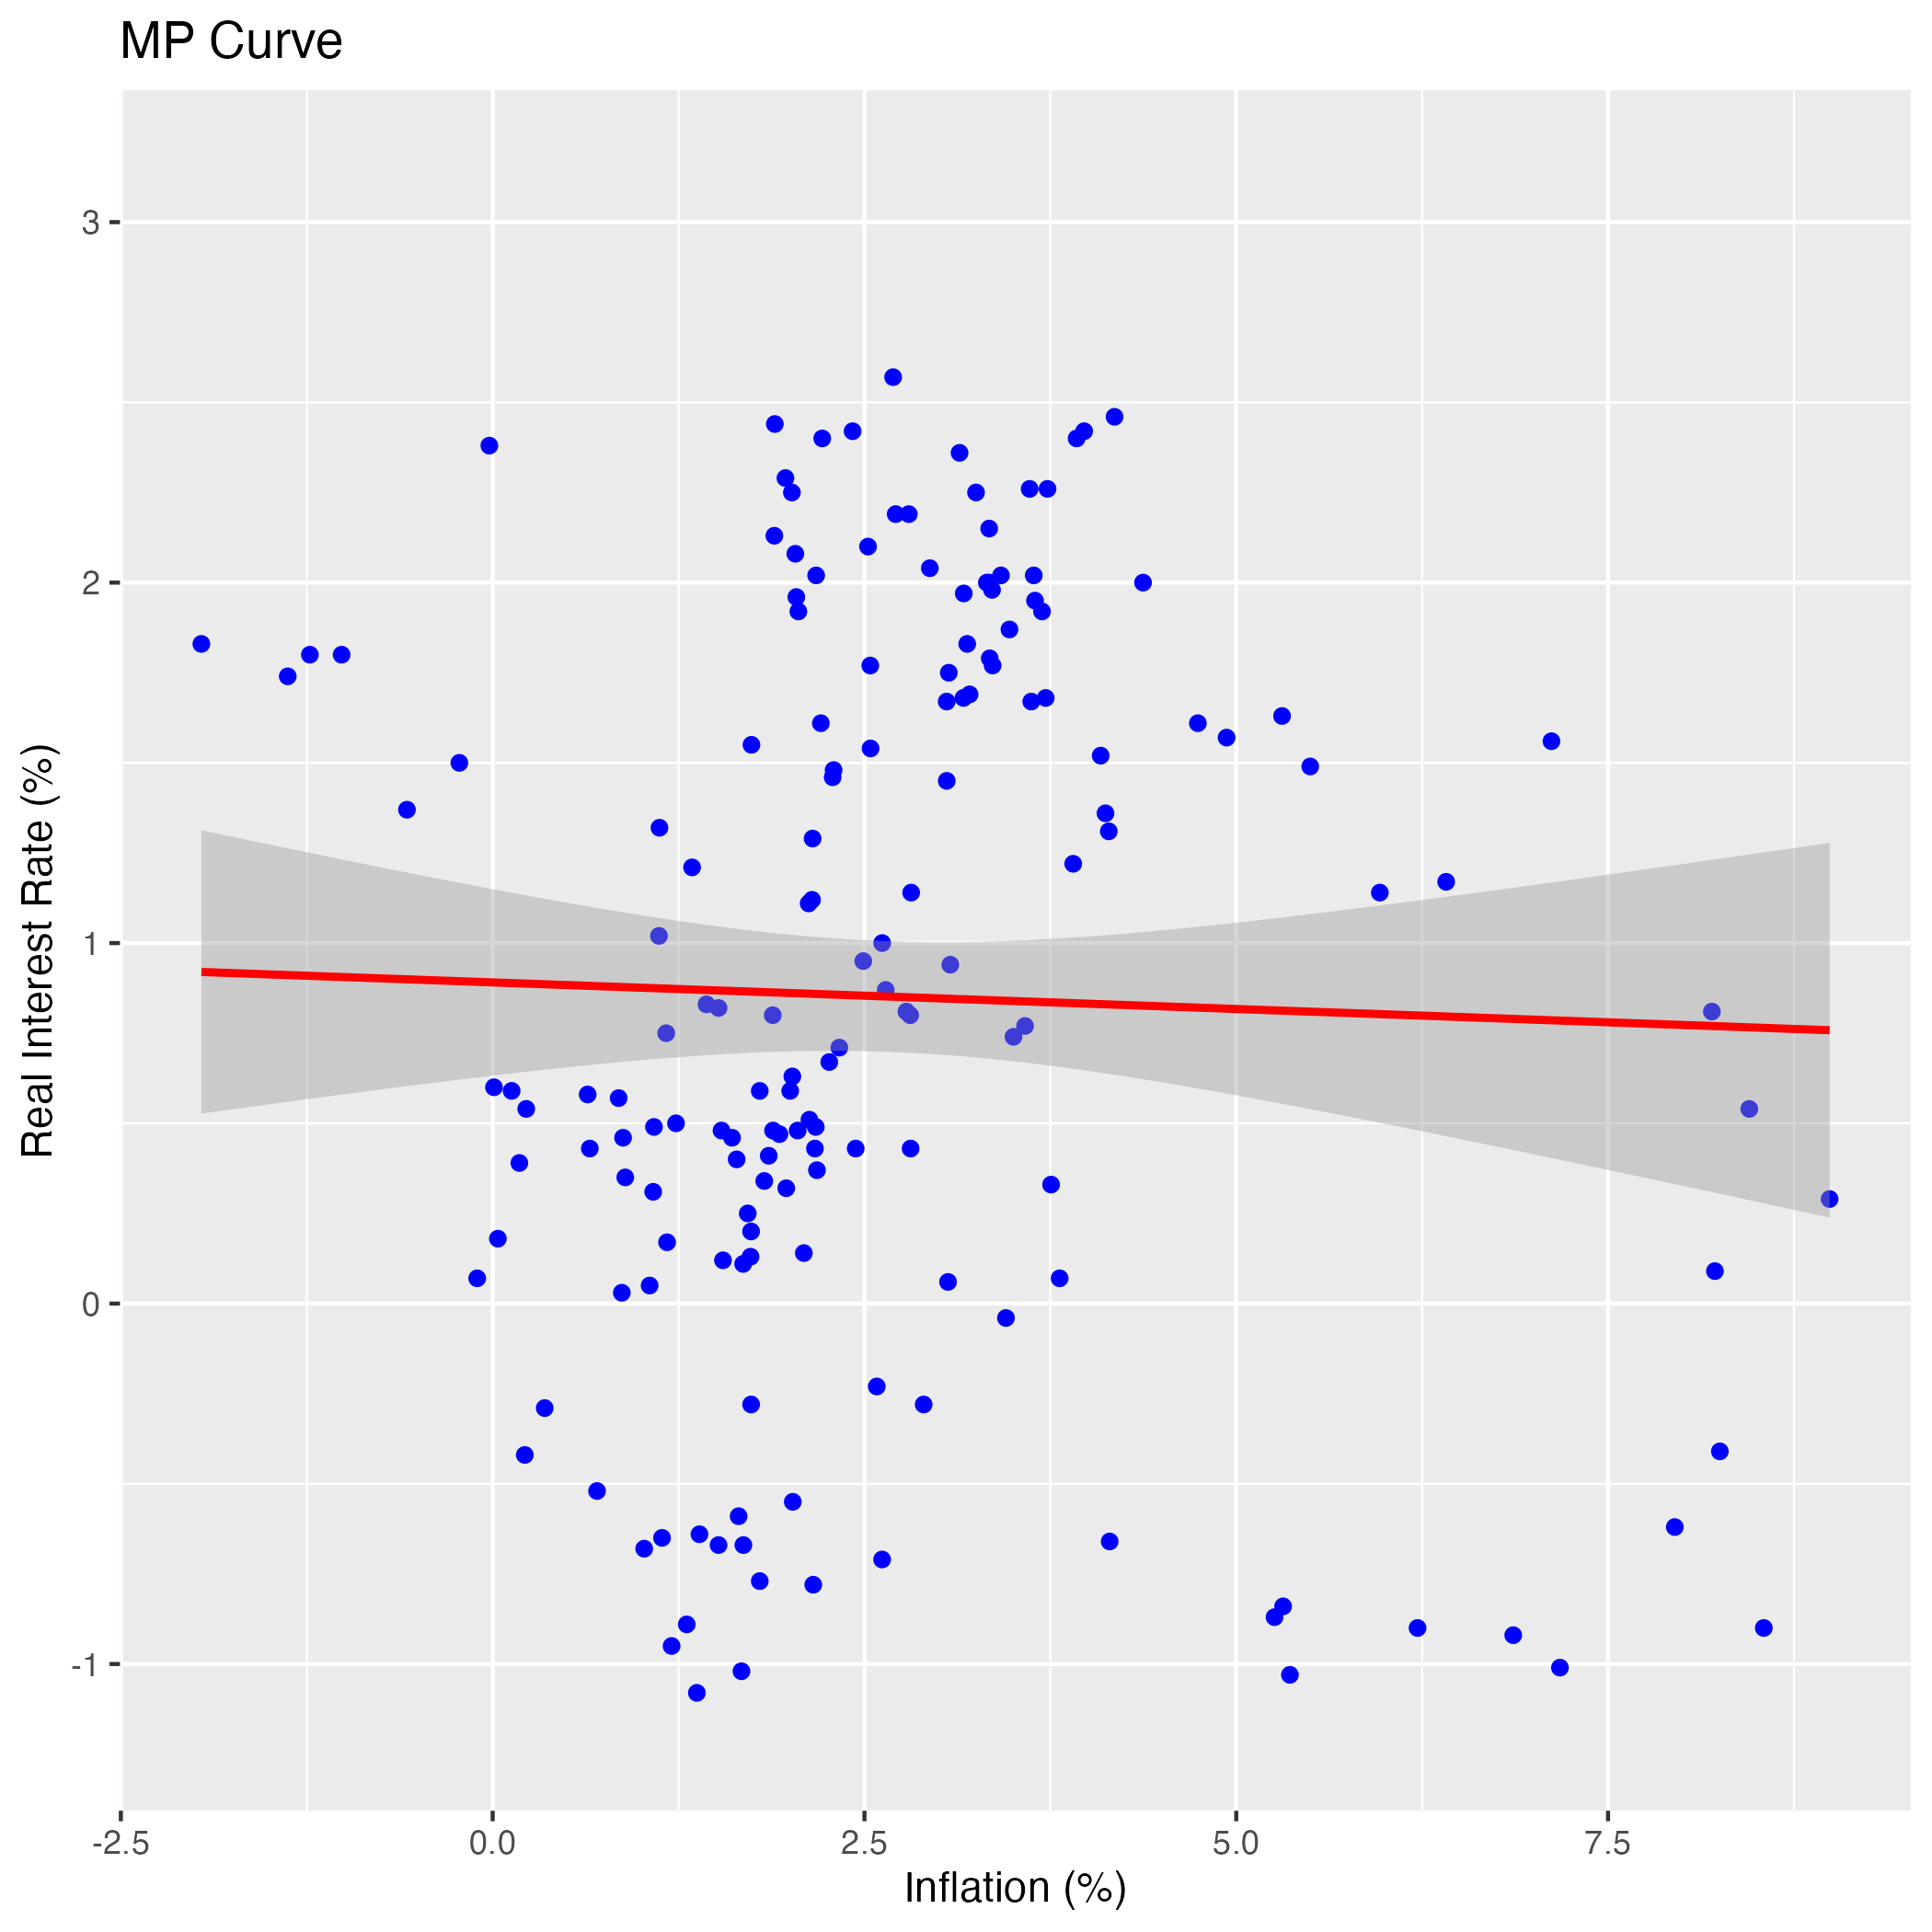
\includegraphics[width=0.8\textwidth]{MP_Curve.png}
\caption{MP Curve}
\end{figure}

\section{The Taylor Rule}
\textbf{Question: Is the Taylor Rule optimal policy? If yes, why? If not, then why is it helpful?}

\subsection{Definition and Formula}
The Taylor Rule provides a guideline for setting interest rates based on inflation and output gaps:
\[
i_t = r^* + \pi_t + 0.5(\pi_t - \pi^*) + 0.5(y_t - y^*)
\]
where $i_t$ is the nominal interest rate, $r^*$ is the real equilibrium interest rate, $\pi_t$ is the inflation rate, $\pi^*$ is the target inflation rate, $y_t$ is the output, and $y^*$ is the potential output.

\subsection{Optimality and Usefulness}
While not always optimal, the Taylor Rule is useful for its simplicity and transparency, helping guide expectations and improve policy credibility.

\section{Dangers of Not Following the Taylor Principle}
\textbf{Question: What are the dangers of failing to follow the Taylor principle when facing high inflation?}

\subsection{Taylor Principle Explanation}
The Taylor Principle states that the central bank should raise nominal interest rates by more than the increase in inflation to stabilize the economy.

\subsection{Consequences of Ignoring the Principle}
Failing to follow the Taylor Principle during high inflation can lead to runaway inflation, as real interest rates fall, boosting aggregate demand and further increasing inflation.

\section{Optimal Stabilization vs. Optimal Disinflation}
\textbf{Question: What’s the difference between optimal stabilization and optimal disinflation? Explain in detail.}

\subsection{Optimal Stabilization}
Optimal stabilization aims to minimize the variance of both inflation and output by responding to shocks in a balanced manner.

\subsection{Optimal Disinflation}
Optimal disinflation focuses on reducing inflation to a lower target level with minimal output loss. This involves a gradual approach to avoid sharp recessions.

\section{Importance of Expectations in Macroeconomics}
\textbf{Question: Explain the importance of expectations in macroeconomics. Why do most standard models assume rational expectations?}

\subsection{Role of Expectations}
Expectations about future economic conditions influence current behavior. For example, if people expect higher inflation, they may spend more now, increasing current inflation.

\subsection{Rational Expectations}
Standard models assume rational expectations, meaning people use all available information to make forecasts, leading to more accurate predictions and efficient markets.

\section{The Lucas Critique}
\textbf{Question: Explain what is the "Lucas critique" and its importance for policy making.}

\subsection{Explanation of Lucas Critique}
The Lucas Critique argues that traditional econometric models fail to account for changes in policy regimes because they don't consider how agents' behavior changes in response to new policies.

\subsection{Importance for Policy Making}
This critique highlights the need for models that incorporate rational expectations and policy impacts on behavior.

\section{Central Bank Preferences and Policy}
\textbf{Question: What are the dangers of having a central bank that aligns perfectly with the preferences of the people? What is a possible solution and why?}

\subsection{Dangers of Alignment}
A central bank too aligned with public preferences may prioritize short-term gains over long-term stability, leading to inflationary policies and economic instability.

\subsection{Solution: Central Bank Independence}
Appointing a conservative central banker who prioritizes inflation control over output stabilization can help mitigate this risk, balancing long-term stability with short-term flexibility.

\section{Conclusion}
Thank you for your attention. This concludes my discussion on monetary policy concepts. I hope this has provided a clear and comprehensive understanding of the topics. If you have any questions, please feel free to ask.

\end{document}
